\documentclass[Analysis/analysis_notes.tex]{subfiles}
\begin{document}
\section{Aula 15 - 24/04/2023}
\subsection{O que esperar}
\begin{itemize}
	\item O Teorema de Weierstrass;
	\item Topologia da Reta;
	\item Teorema de Borel-Lebesgue.
\end{itemize}
\subsection{Resultados Avan\c cados de Continuidade - Parte 2.}
Um resultado que vale ser mencionado \'e a caracteriza\c c\~ao de continuidade via limites:
\begin{theorem*}
	Seja D um subconjunto dos reais, $f:D\rightarrow \mathbb{R}$ e p um ponto de D. A fun\c c\~ao f \'e cont\'inua em p se, e somente
	se, para toda sequ\^encia $\{x_{n}\}$ em D com $x_{n}\overbracket[0pt]{\longrightarrow}^{n\to \infty}p,$ existe o limite $\lim_{n\to \infty}f(x_{n}).$
\end{theorem*}
\begin{crl*}
	Seja D um subconjunto de $\mathbb{R}, f:D\rightarrow \mathbb{R} $ e p um ponto de D. A fun\c c\~ao f \'e cont\'inua se, e somente
	se, para toda sequ\^encia $\{x_{n}\}$ em D com $x_{n}\overbracket[0pt]{\longrightarrow}^{n\to \infty}p$ temos $f(x_{n})\overbracket[0pt]{\longrightarrow}^{n\to \infty}f(p).$
\end{crl*}
Vamos relembrar os resultados vistos na aula anterior.
\begin{theorem*}
	Seja $f:D_{f}\rightarrow \mathbb{R}$ uma fun\c c\~ao cont\'inua e $\overline{x}\in D_{f}$ tal que $f(\overline{x})>0(f(\overline{x})<0).$
	Ent\~ao, existe $\delta>0$ tal que $f(x)>0(f(x)<0)$ para todo $x\in D_{f}$ e $x\in(\overline{x}-\delta, \overline{x}+\delta).$
\end{theorem*}
\begin{proof*}
	Como f \'e cont\'inua em $\overline{x},$ dado $\varepsilon = f(\overline{x}) >0$, exsite $\delta > 0$ tal que
	$$
		x\in D_{f}, x\in(\overline{x}-\delta, \overline{x}+\delta) \Rightarrow f(x)\in (f(\overline{x})-\varepsilon, f(\overline{x})+\varepsilon)) =
		(0, 2f(\overline{x})).
	$$
	Isto prova o resultado. \qedsymbol
\end{proof*}
O pr\'oximo \'e o Teorema do Anulamento.
\begin{theorem*}
	Se $f:[a,b]\rightarrow \mathbb{R}$ \'e cont\'inua e $f(a)<0<f(b) (f(a)>0>f(b)),$ ent\~ao existe $\overline{x}\in(a, b)$ tal que $f(\overline{x}) =0.$
\end{theorem*}
\begin{proof*}
	Faremos apenas o caso $f(a)<0<f(b).$ Seja
	$$
		A = \{x\in[a,b]:f(s)>0 \forall s\in[x, b].\}
	$$
	Note que $A\neq\emptyset$ e $A\subseteq{[a, b]}.$ Seja $z =\inf{A}$. Pelo Teorema da Conserva\c c\~ao de Sinal,
	$z\in(a, b)$ e $z\not\in A.$ Destarte, $f(z)\leq{0}.$ Por outro lado, do Teorema da Compara\c c\~ao, $f(z)=
		\lim_{x\to z^{+}}f(x)\geq{0}$, pois como $x > z,$ x \'e um elemento de A, o que torna $f(x)>0$. Portanto, f(z)=0.
\end{proof*}
A seguir, veremos o Teorema do Valor Intermedi\'ario.
\begin{theorem*}
	Seja $f:[a, b]\rightarrow \mathbb{R}$ uma fun\c c\~ao cont\'inua e tal que  $f(a)<f(b)(f(a)>f(b))$. Se $f(a)<k<f(b)(f(a)>k>f(b)),$
	ent\~ao existe $\overline{x}\in(a, b)$ tal que $f(\overline{x})=k.$
\end{theorem*}
\begin{proof*}
	Considere a fun\c c\~ao $g(x)=f(x)-k.$ Ent\~ao, $g:[a, b]\rightarrow \mathbb{R}$ \'e cont\'inua, $g(a)<0, g(b)>0$
	e do Teorema do Anulamento, existe $\overline{x}\in[a, b]$ tal que $g(\overline{x})=0.$ Portanto, $f(\overline{x})=k.$\qedsymbol
\end{proof*}
As vers\~oes an\'alogas ficam como exerc\'icio para o estudante.
A seguir, um dos resultados fundamentais da an\'alise \'e apresentado, o Teorema de Weierstrass
\begin{theorem*}
	Se $f:[a, b]\rightarrow \mathbb{R}$ for cont\'inua, existir\~ao p, q em $[a, b]$ tais que
	$$
		f(p)\leq f(x)\leq f(q),\quad \forall x\in[a,b]
	$$
\end{theorem*}
\begin{proof*}
	Vamos mostrar que a imagem da f \'e limitada, incialmente. Se ela n\~ao fosse limitada, dado n natural, existiria $x_{n}\in[a, b]$
	tal que para $x_{0}\in[a, b]$ e $|f(x_{n})| > \max{\{n, |f(x_{n-1})|\}}, n\in \mathbb{N}^{\times}.$ Seja $A=\{x_{n}:n\in \mathbb{N}\}$.
	Com aquele $x_{0},$ obtemos $x_{1}\in[a, b]$ tal que $|f(x_{1})| > 1 + |f(x_{0})|, |f(x_{2})| > 1 + |f(x_{1})| > 2 + |f(x_{0})|.$
	Indutivamente, $|f(x_{n})| > n + |f(x_{0})|.$ Segue que $A\subseteq{[a, b]}$ tem um ponto de acumula\c c\~ao $r\in[a, b].$

	Como f \'e con\t'inua em r, existe $\delta > 0 tal que,$
	$$
		x\in(r-\delta , r+\delta )\cap[a, b] = B \Rightarrow |f(x)-f(r)|<1.
	$$

	Obtemos que f(B) \'e limitado e cont\'em infinitos pontos de f(A), uma contradi\c c\~ao. Logo, a imagem de f Im(f) \'e limitada.

	Seja $m=\inf{\{f(x):x\in[a, b]\}}$. Ent\~ao, $f(x)\geq m$ para todo x em $[a, b].$ Se f n\~ao \'e constante, m ser\'a ponto de
	acumula\c c\~ao do conjunto $\{y\in{Im(f)}: y > m\}$. Tome $x_{0}\in[a, b]$ tal que $0 < f(x_{0}) - m$ e $x_{k}\in[a, b]$
	tal que $0 < f(x_{0}) - m < \min{\{\frac{1}{k}, f(x_{k-1})-m\}}$ para k em $\mathbb{N}^{\times}.$

	O conjunto $A = \{x_{k}: k\in \mathbb{N}\}$ \'e infinito e limitado, portanto A tem um ponto de acumula\c c\~ao p. Como f \'e cont\'inua
	em p, para cada n em $\mathbb{N}^{\times},$ existe $\delta_{n} > 0$ tal que
	$$
		x\in[a, b], |x-p|<\delta_{n} \Rightarrow |f(x)-f(p)|<\frac{1}{n}.
	$$
	Em particular, escolha $x_{k}$ em A com $k>n$ e tal que $|x_{k}-p|<\delta_{n},$
	$$
		m-\frac{1}{n} < f(x_{k})-\frac{1}{n}<f(p)<f(x_{k}) + \frac{1}{n} < m + \frac{1}{n} + \frac{1}{k} < m + \frac{2}{n}.
	$$
	Assim, f(p) = m. A afirmativa segue de $-\inf{\{Im(-f)\}} = \sup\{Im(f)\}$ \qedsymbol
\end{proof*}
\begin{crl*}
	Seja $f:[a, b]\rightarrow \mathbb{R}$ cont\'inua. Se
	$$
		m=\min{\{f(x):x\in[a, b]\}},\quad M = \max{\{f(x):x\in[a, b]\}},
	$$
	ent\~ao
	$$
		Im(f) = f([a, b]) = [m, M].
	$$
\end{crl*}

\subsection{Topologia da Reta}
\subsubsection{Texto de Motiva\c c\~ao}
A topologia da reta estuda a estrutura dos conjuntos de pontos na reta real, analisando as propriedades topológicas dos mesmos. A reta real é um espaço topológico particularmente interessante devido à sua simplicidade e conexão com outras áreas da matemática, como análise e álgebra.

Considere a sucessão de números reais $(x_n)$. Quando é que podemos dizer que essa sucessão converge para um número real $x$? A topologia da reta nos ajuda a entender a convergência e a continuidade de funções reais.

\begin{center}
	\begin{tikzpicture}
		\draw[->] (-0.5,0) -- (5,0);
		\draw[->] (0,-0.5) -- (0,2);
		\node at (5.2,0) {$x$};
		\node at (0,2.2) {$y$};

		\foreach \x in {1,2,3,4}
		\draw (\x,1pt) -- (\x,-1pt) node[anchor=north] {$x_\x$};

		\draw[dashed] (1,0) -- (1,1);
		\draw[dashed] (2,0) -- (2,0.5);
		\draw[dashed] (3,0) -- (3,0.75);
		\draw[dashed] (4,0) -- (4,0.875);

		\filldraw (1,1) circle (1.5pt);
		\filldraw (2,0.5) circle (1.5pt);
		\filldraw (3,0.75) circle (1.5pt);
		\filldraw (4,0.875) circle (1.5pt);
	\end{tikzpicture}
\end{center}

A topologia da reta também lida com conceitos como limites e fronteiras de conjuntos. Por exemplo, qual é o limite superior de um conjunto $A \subseteq \mathbb{R}$? E qual é a fronteira de um conjunto aberto?
Uma ilustra\c c\~ao de conjunto aberto \'e o intervalo (a, b):

\begin{center}
	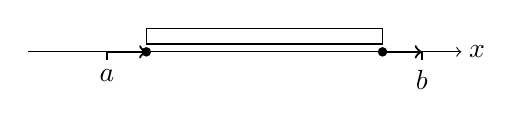
\begin{tikzpicture}
		\draw[->] (-0.5,0) -- (5,0);
		\node at (5.2,0) {$x$};

		\draw (1,0.1) rectangle (4,0.3);
		\draw[thick] (0.5,0) -- (0.5,-0.1) node[below] {$a$};
		\draw[thick] (4.5,0) -- (4.5,-0.1) node[below] {$b$};

		\draw[<-, thick] (1,0) -- (0.5,0);
		\draw[->, thick] (4,0) -- (4.5,0);

		\fill[white] (1,0) circle (1.5pt);
		\fill[white] (4,0) circle (1.5pt);
		\filldraw (1,0) circle (1.5pt);
		\filldraw (4,0) circle (1.5pt);
	\end{tikzpicture}
\end{center}

Um espaço topológico é um conjunto $X$ juntamente com uma coleção de subconjuntos $\tau$ que satisfazem certas propriedades. Estes subconjuntos são chamados de conjuntos abertos. Na reta real, podemos definir a topologia usual usando intervalos abertos.
Aqui est\'a o c\'odigo representando um conjunto aberto da reta real, tal como seus pontos de fronteira. A barra representa o lugar em que
os pontos est\~ao, as setas saindo de a e b indicam que os pontos n\~ao est\~ao inclusos no conjunto, tornando-o aberto.

\begin{center}
	\begin{tikzpicture}
		\draw[->] (-0.5,0) -- (5,0);
		\node at (5.2,0) {$x$};

		\draw[pattern=north east lines, pattern color=green] (1,0.1) rectangle (4,0.3);
		\draw[thick] (0.5,0) -- (0.5,-0.1) node[below] {$a$};
		\draw[thick] (4.5,0) -- (4.5,-0.1) node[below] {$b$};

		\draw[<-, thick] (1,0) -- (0.5,0);
		\draw[->, thick] (4,0) -- (4.5,0);

		\filldraw (1,0) circle (1.5pt);
		\filldraw (4,0) circle (1.5pt);
	\end{tikzpicture}
\end{center}

Na reta real, um conjunto é aberto se, para cada ponto $x$ no conjunto, existe um intervalo aberto contendo $x$ e inteiramente contido no conjunto. Já um conjunto fechado é aquele cujo complementar é aberto.
Outras ideias importantes s\~ao de conectividade e compacidade.

Um conjunto é dito conexo se não puder ser dividido em dois conjuntos abertos disjuntos. Na reta real, intervalos são exemplos de conjuntos conexos.

Um conjunto é compacto se todo subconjunto aberto que o cobre possui um subconjunto finito que também o cobre. Na reta real, intervalos fechados e limitados são exemplos de conjuntos compactos.
O Teorema de Bolzano-Weierstrass afirma que toda sequência infinita de pontos em um conjunto compacto possui uma subsequência convergente. Como esperado,
ele possui aplica\c c\~oes diretas na converg\^encia de sequ\^encias e fun\c c\~oes juntando com os resultados que vimos.

Suponha que você tenha uma sequência infinita de pontos dentro de um intervalo fechado e limitado na reta real. O Teorema de Bolzano-Weierstrass garante que sempre é possível encontrar uma subsequência desses pontos que converge para algum ponto dentro desse intervalo. Isso significa que, por mais ``espalhados" que esses pontos possam estar, sempre haverá algum padrão de convergência.

Portanto, a topologia da reta fornece uma base sólida para o estudo de propriedades topológicas e estruturas dos conjuntos de pontos na reta real. Aprofundemo-nos
em seu estudo.
\subsubsection{Abertos, Fechados, Compactos e Conexos}
\begin{def*}
	Seja A um subconjunto de $\mathbb{R}.$
	\begin{itemize}
		\item[1)] Um ponto a de A \'e dito interior a A se existe um r positivo tal que $(a-r, a+r)\subseteq{A}.$
		\item[2)] O conjunto A \'e aberto se todos os seus pontos s\~ao interiores.
		\item[3)] O conjunto A \'e fechado em $\mathbb{R}$ se seu complementar \'e aberto.
		\item[4)] O interior de A, $A^{\circ},$ \'e o conjunto dos pontos interiores a A.
		\item[5)] O fecho $\overline{A}$ de A \'e a interse\c c\~ao de todos os fechados que cont\'em A.
	\end{itemize}
\end{def*}
\'E poss\'ivel mostrar que intervalos abertos s\~ao conjuntos abertos (tome $r=\min{\{b-x, x-a\}}, x\in(a, b)$), intervalos fechados s\~ao conjuntos fechados, etc.
\begin{theorem*}
	Seja $\Lambda $ um conjunto e $\{A_{\lambda }\}_{\lambda \in\Lambda } $ uma fam\'ilia de conjuntos.
	\begin{itemize}
		\item[1)] Se cada $A_{\lambda }$ \'e aberto, $\bigcup_{\lambda\in\Lambda  }^{}{A_{\lambda }}$ \'e aberto.
		\item[2)] Se cada $A_{\lambda }$ \'e aberto e $\Lambda $ \'e finito, $\bigcap_{\lambda \in\Lambda }^{}{A_{\lambda }}$
		      \'e aberto.
		\item[3)] Se cada $A_{\lambda }$ \'e fechado, $\bigcap_{\lambda \in\Lambda }^{}{A_{\lambda }}$ \'e fechado.
		\item[4)] Se cada $A_{\lambda }$ \'e fechado e $\Lambda $ \'e um conjunto finito, $\bigcup_{\lambda \in\Lambda }^{}{A_{\lambda }}$
		      \'e fechado.
	\end{itemize}
	(1) Como cada $A_{\lambda }$ \'e composto de todos os pontos interiores, $\bigcup_{\lambda \in\Lambda }^{}{A_{\lambda }}$ tamb\'em tem
	todos os seus pontos como pontos interiores. Portanto, $\bigcup_{\lambda \in\Lambda }^{}{A_{\lambda }}$ \'e aberto.

	(2) Tome x em $\bigcap_{\lambda \in\Lambda }^{}{A_{\lambda }}.$ Ent\~ao, existe um $r_{\lambda }$ tal que $(x-r_{\lambda }, x+r_{\lambda })\subseteq{A_{\lambda }}.$
	Como temos um n\'umero finito de abertos, tome $r\coloneqq \min{\{r_{\lambda }:\lambda \in\Lambda \}}$. Ent\~ao,
	$$
		(x-r, x+r)\subseteq{(x-r_{\lambda },x+r_{\lambda })}\subseteq{A}.
	$$
	Portanto, $\bigcap_{\lambda \in\Lambda }^{}{A_{\lambda }}$ \'e aberto.

	Os itens (3) e (4) seguem utilizando os itens (1) e (2) e as leis de De Morgan (complementar da uni\~ao \'e a interse\c c\~ao dos complementares, etc.). \qedsymbol
\end{theorem*}
\begin{example}
	Mostramos que intervalos abertos s\~ao abertos. N\~ao apenas isso, mas o interior de [a, b] \'e (a, b).
\end{example}
\begin{example}
	O interior $A^{\circ}$ de A \'e o maior aberto que cont\'em A. O fecho $\overline{A}$ de A \'e o menor fechado que cont\'em A.
\end{example}
\begin{theorem*}
	Todo subconjunto aberto A de $\mathbb{R}$ se exprime, de maneira \'unica, como uni\~ao enumer\'avel de intervalos abertos disjuntos.
\end{theorem*}
\begin{proof*}
	Primeiramente, note que se $\Lambda $ \'e um conjunto, para cada $\lambda, I_{\lambda }=(a_{\lambda }, b_{\lambda })$ \'e um intervalo
	e $p\in\bigcap_{\lambda \in\Lambda }^{}{I_{\lambda }}$, ent\~ao $\bigcup_{\lambda \in\Lambda }^{}{I_{\lambda }}=(a, b),$ sendo
	$a = \inf_{\lambda \in\Lambda }a_{\lambda }, b = \sup_{\lambda \in\Lambda }b_{\lambda }.$ De fato, \'e claro que $\bigcup_{\lambda \in\Lambda }^{}{I_{\lambda }}\subseteq{(a, b)}$.
	Para provar a outra inclus\~ao, note que $p\in(a, b)$ e se $x\in(a, b), x\leq p ou x > p.$ Agora,
	\begin{align*}
		 & (1) \text{ Se }  x\leq p, a = \inf_{\lambda \in\Lambda }a_{\lambda } < x \Rightarrow \exists \mu_{1}\in\Lambda: a_{\mu_{1}}<x\leq p < b_{\mu_{1}} \\
		 & (2) \text{ Se } x > p, b=\sup_{\lambda \in\Lambda }b_{\lambda } < x \Rightarrow \exists \mu_{2}\in\Lambda: a_{\mu_{2}} < p < x < b_{\mu_{2}}.
	\end{align*}
	Em qualquer caso,  $x\in \bigcup_{\lambda \in\Lambda }^{}{I_{\lambda }}.$

	Para terminar, dado x em A, seja $I_{x}$ a uni\~ao de todos os abertos contidos em A que cont\'em x. Segue que
	\begin{itemize}
		\item[1)] $I_{x} = (a_{x}, b_{x})\subseteq{A};$
		\item[2)] Se x, y s\~ao pontos de A, ou $I_{x}\cap I_{y}=I_{x} = I_{y},$ ou $I_{x}\cap I_{y} = \emptyset$;
		\item[3)] $\bigcup_{x\in A}^{}{I_{x}} = A.$
	\end{itemize}
	Tomando para cada intervalo da decomposi\c c\~ao um \'unico racional, vemos que A pode ser escrito como uni\~ao enumer\'avel de
	intervalos disjuntos. Para ver que esta decomposi\c c\~ao \'e \'unica, basta notar que cada intervalo aberto de uma tal decomposi\c c\~ao
	est\'a contido em algum dos $I_{x}$ e n\~ao pode ser distinto de $I_{x}.$ \qedsymbol
\end{proof*}
\begin{crl*}
	Se I \'e um intervalo aberto e $I = A\cup B,$ em que A e B s\~ao conjuntos abertos e disjuntos, ent\~ao um desses conjuntos \'e vazio.
\end{crl*}
\end{document}
